\documentclass[tikz]{standalone}

\usepackage{graphicx}
\usepackage{tikz}
\usetikzlibrary{arrows.meta, automata, positioning, quotes}

\tikzstyle{every picture} = [node distance=1.3cm]


\begin{document} 
	%\begin{center}
		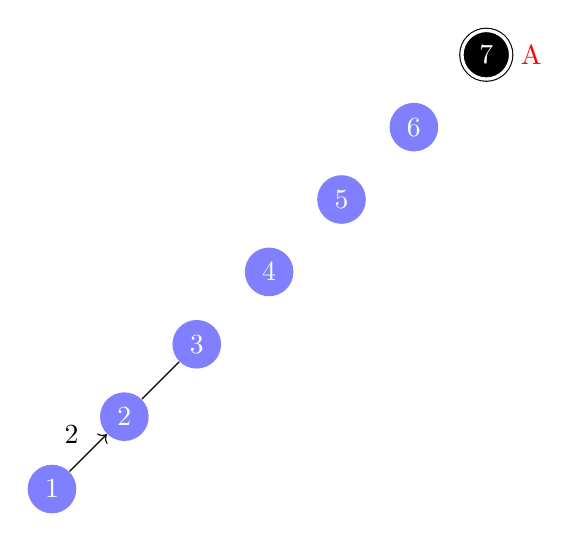
\begin{tikzpicture} 
			\node (node 1) [circle, double, double distance =1.2pt,text=white,fill=blue!50,] {1};
			\node (node 2) [circle, double, double distance =1.2pt,text=white,fill=blue!50,above right of= node 1] {2};
			\node (node 3) [circle, double, double distance =1.2pt,text=white,fill=blue!50,above right of= node 2] {3};
			\node (node 4) [circle, double, double distance =1.2pt,text=white,fill=blue!50,above right of= node 3] {4};
			\node (node 5) [circle, double, double distance =1.2pt,text=white,fill=blue!50,above right of= node 4] {5};
			\node (node 6) [circle, double, double distance =1.2pt,text=white,fill=blue!50,above right of= node 5] {6};
			\node (node 7) [circle, double, double distance =1.2pt,text=white,fill= ,above right of= node 6,label={[red]right:A}, draw=] {7};
			\path (node 1) edge[->,"2",] (node 2);
			\path (node 2) edge[-,] (node 3);
		\end{tikzpicture}
	%\end{center}
\end{document}
